\chapter{Ethereum: Sviluppo di applicazioni decentralizzate}

Seguendo la divisione a tre strati: di concetti, implementazioni e istanze definita fin dall'inizio del lavoro, in questo capitolo verrà affrontato l'aspetto dell'implementazione nel caso concreto della piattaforma Ethereum. I concetti spiegati fino a questo punto costituiscono un base decisionale, un punto di partenza per scegliere le implementazioni che meglio si adottano alle proprie necessità. I concetti presentati finora possono essere visti come una sorta di contenitore aperto da cui è possibile “pescare” le componenti concettuali da implementare a seconda delle funzionalità dell’applicazione reale. 

Importante sottolineare che lo stato dell'arte delle blockchain limita l’utilità di descrivere in dettaglio le implementazioni concrete. Questa affermazione deriva dal contesto attuale, le blockchain nonostante non siano più definibili come una tecnologia fra le più recenti in confronto alle tempistiche nel settore informatico, generalmente non hanno raggiunto una stabilità sufficiente. Usando la terminologia presente nelle analisi e predizioni annuali condotte dalla Gartner\footfullcite{gart} la blockchain si trova attualmente sulla via di uscita dal cosiddetto "hype cycle"\footfullcite{gart2016} \smallskip \footfullcite{gart2018}. Una metodologia usata per rappresentare la maturità, l'adozione e l'applicazione di nuove tecnologie.

\begin{figure}[H]
\centering
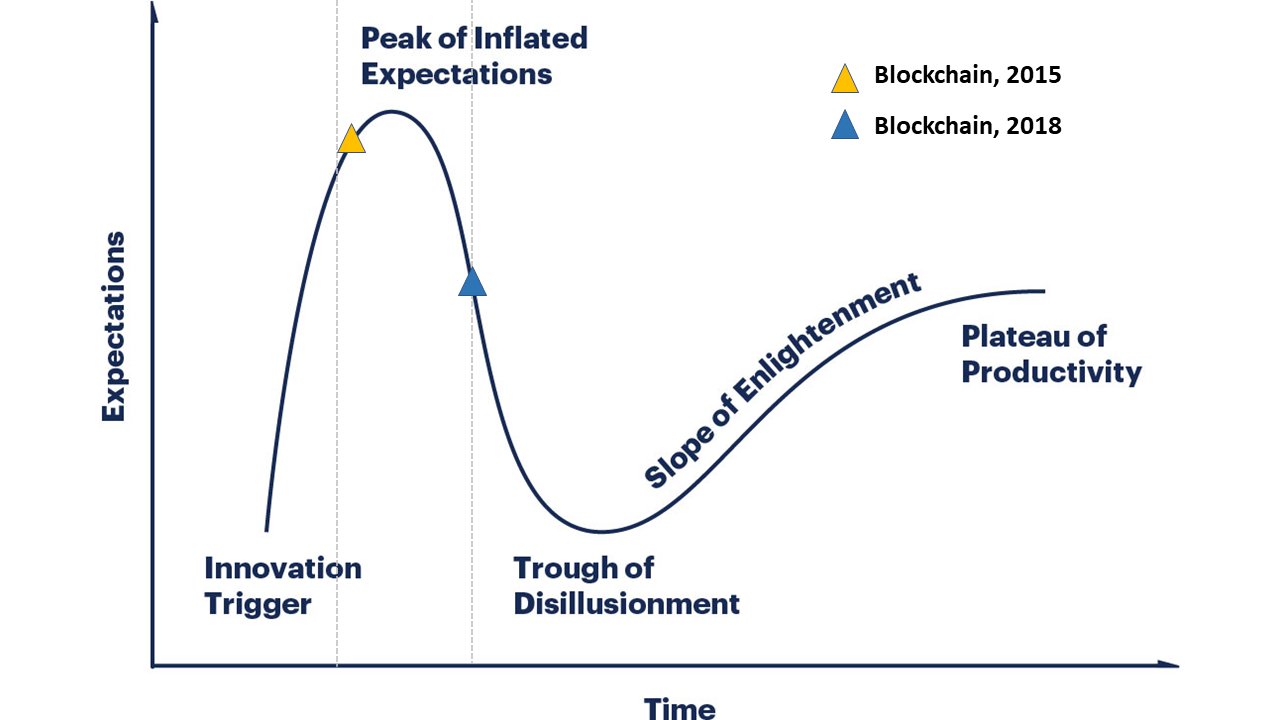
\includegraphics[width=1\textwidth]{immagini/blockchainHype.png}
\caption{Blockchain: Hype cycle}
\label{fig:mesh7}
\end{figure}

La situazione può essere vista come un contesto variabile, di continuo sviluppo con l’emergere di nuove implementazioni, piattaforme e applicazioni. Una ricerca spesso finalizzata al miglioramento e adozione delle nuove tecniche per contrastare le limitazioni attuali del sistema ma pur sempre una situazione, qual è quella presente, in continuo mutamento caratterizzata dall'instabilità e in alcuni casi, cambiamenti radicali. Tuttavia, questo non pregiudica l’utilità delle cose dette finora in quanto si tratta di concetti fondamentali che, nel caso peggiore, possono servire anche per comprendere le scelte e gli sviluppi futuri. 

La scelta di Ethereum come sistema da presentare, collegato alla successiva costruzione di un’applicazione nel capitolo successivo è stata fatta seguendo tra le altre, queste motivazioni: di stabilità, sviluppo e innovazione. Viene perseguita l'idea legata alla correlazione tra il successo e la popolarità di un sistema misurata tenendo conto del numero di partecipanti e sviluppatori coinvolti, gli strumenti di sviluppo messi a disposizione e il loro grado di maturità, la frequenza di aggiornamenti e l’interesse della comunità ed enti pubblici e privati con i relativi rischi connessi. Un insieme di fattori che le nuove implementazioni dovranno cercare di raggiungere per attrarre gli utenti e gli sviluppatori ai loro sistemi. Al momento dello scrivere la piattaforma Ethereum è il sistema più sviluppato sotto l’aspetto di sviluppo delle applicazioni decentralizzate.

\section{Implementazione Ethereum}

Ethereum è una di piattaforma di sviluppo delle applicazioni decentralizzate basata sulla tecnologia blockchain pubblica e open-source.

La novità principale è data dalla possibilità di programmazione in maniera Turing Completa. Si tratta dunque, di una blockchain programmabile con un linguaggio chiamato Solidity attraverso cui è possibile esprimere qualsiasi algoritmo esprimibile con altri linguaggi di programmazione universali. Questi programmi scritti e compilati all’interno della blockchain prendono il nome di “Smart Contracts” e si comportano come dei contratti veri e propri. In rapporto ai loro corrispettivi tradizionali i termini contrattuali non sono definiti usando un linguaggio legale ma direttamente il codice dei programmi (chiamati appunto contratti). Gli smart contracts, permettono quindi l’impementazione della logica delle transazioni e inoltre permettono la disintermediazione tra le parti interessate grazie ai concetti che guidano le blockchain. 

Riassumendo, la visione del progetto Ethereum è quella di creare un computer decentralizzato permanente e autosufficiente in grado di resistere ai tentativi di censura. Dal punto di vista della programmazione, nella figura 3.2 è rappresentato il flusso relativo all’architettura di un’applicazione blockchain.

\begin{figure}[H]
\centering
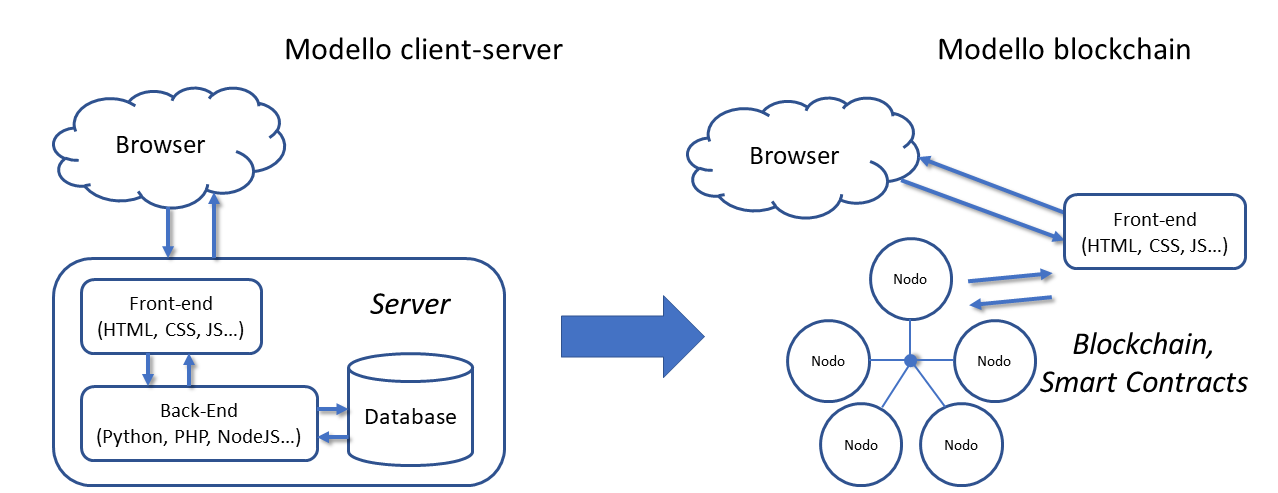
\includegraphics[width=1\textwidth]{immagini/architetturav1.png}
\caption{Blockchain: Modello dell'architettura}
\label{fig:mesh8}
\end{figure}

In relazione al classico modello client-server, nel modello decentralizzato lo strato back-end è direttamente implementato nella blockchain attraverso gli smart contract situati direttamente sulla blockchain che a sua volta corrisponde a una base di dati con storia completa e distribuita su tutti i nodi. L’esecuzione della logica dei contratti avviene grazie alla macchina virtuale Ethereum (EVM) eseguita da ciascun nodo della rete.


In questo capitolo verranno ripresi i concetti presentati e le loro implementazioni concrete con le relative modifiche ed espansioni. Nella vista di insieme si parlerà di:

\begin{itemize}
\item Espansione del concetto di transazione
\item Struttura dati Patricia trees come espansione di Merkle trees
\item Funzioni hash Keccak
\item Sistema di consenso con il passaggio da Proof of Work in Ethereum Metropolis  a Proof of Stake nella versione Constantinople
\end{itemize}

Caratteristiche: 
- Permessi: è una blockchain pubblica, decentralizzata\\
- Hash: funzione di hash keccak256\\
- Struttura dati: Merkle Trees - patricia trees\\
- Sistema di consenso PoW\\
- Smart contracts\\
-- DA FARE\\

\subsection{Transazioni}

\subsection{Patricia Trees}

\begin{figure}[H]
\centering
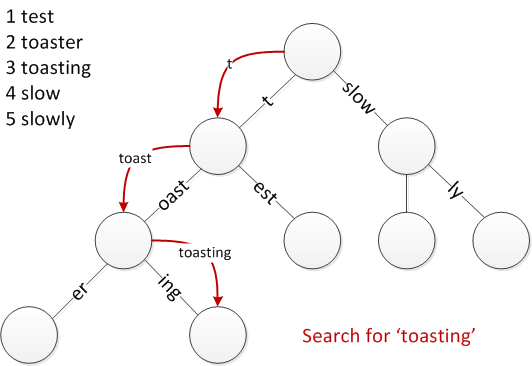
\includegraphics[width=1\textwidth]{immagini/patricia_trie.png}
\caption{Struttura di patricia trie}
\label{fig:mesh6}
\end{figure}

\subsection{Ethereum Metropolis e Constantinople}

Qui scrivo del consenso e della transizione da PoW a PoS
Magari anche forks?

\section{Smart Contracts}

\subsection{Solidity}

\subsection{Ethereum Virtual Machine}

\subsection{Gas}

\section{Data storage}